% All figures below were checked against the repository (master).
% ======================================================================
% (1) Ch 4 "Use Case Diagram": replaces the current Figure 4.1
% ======================================================================
\begin{figure}[htbp]
\centering
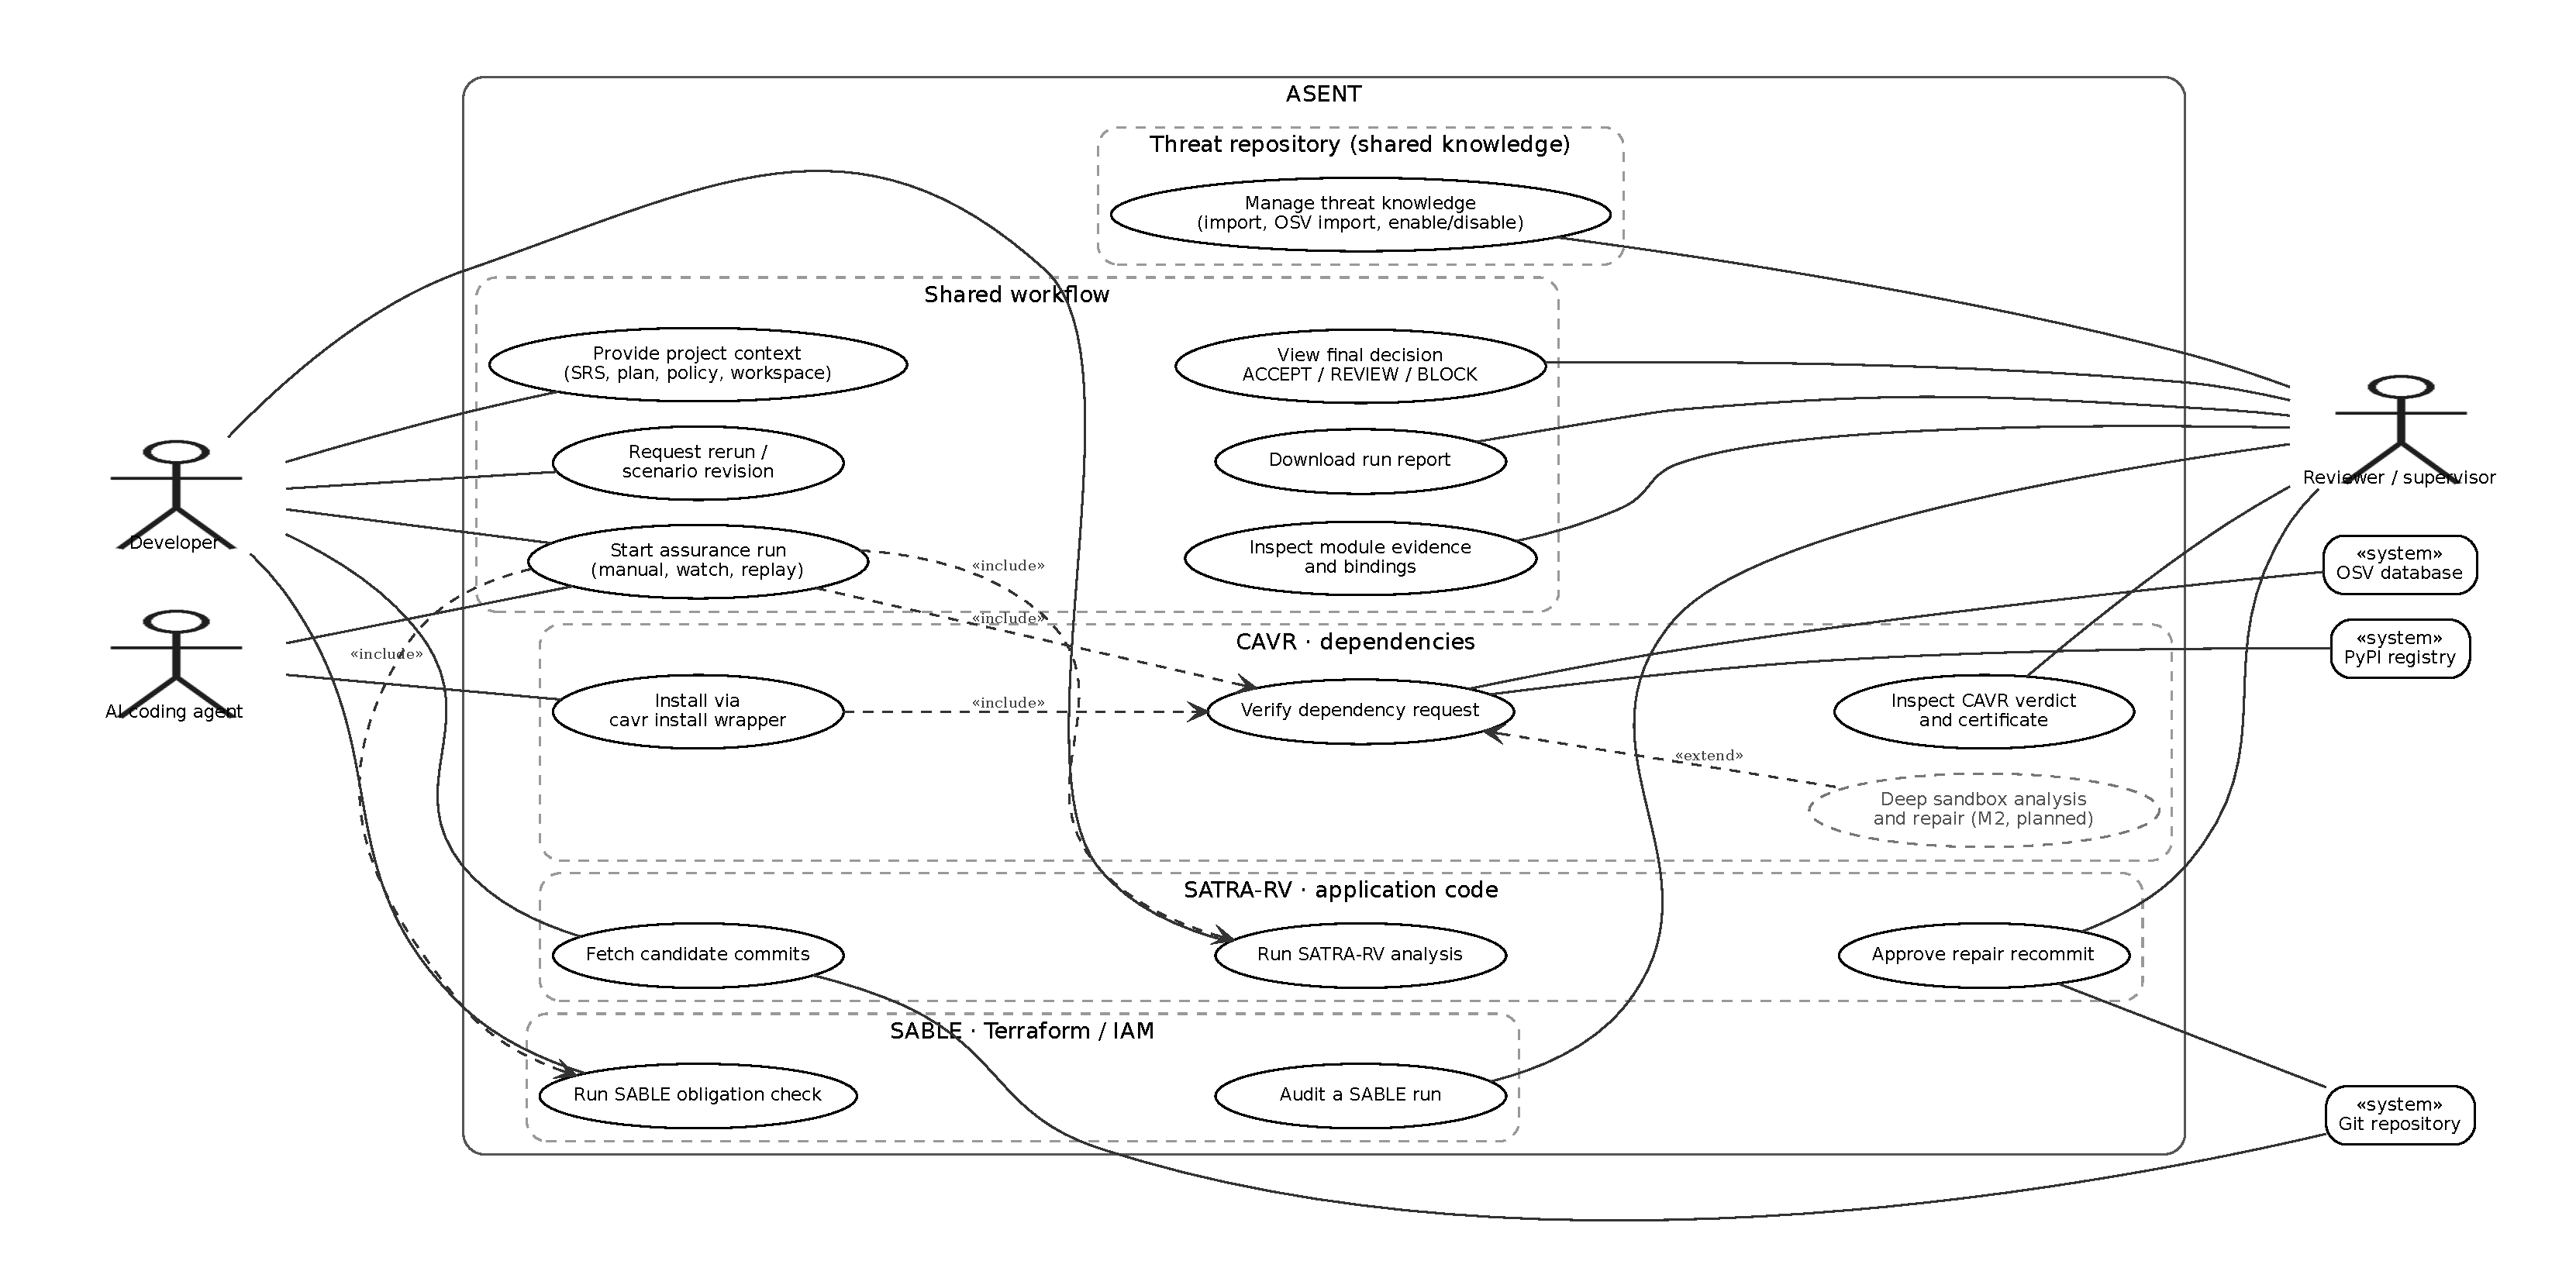
\includegraphics[width=\textwidth]{figures/diagrams/usecase.pdf}
\caption{ASENT use cases. Actors are the developer, the AI coding agent and the reviewer; PyPI, OSV and the Git repository are external systems. The dashed use case is planned for M2.}
\label{fig:asent-usecase}
\end{figure}

Figure~\ref{fig:asent-usecase} shows who uses ASENT and for what; every use case corresponds to a route of the local API (\texttt{/api/runs}, \texttt{/api/cavr}, \texttt{/api/satra}, \texttt{/api/sable}, \texttt{/api/threat-repository}) or to the \texttt{cavr install} wrapper. The developer provides the project context, starts assurance runs and module runs; the AI coding agent starts runs through the watch/replay adapters and installs packages through the wrapper; the reviewer inspects decisions, evidence and certificates, approves SATRA repair recommits, audits SABLE runs and manages the shared threat knowledge. Starting a run \emph{includes} the applicable module analyses, and installing through the wrapper always \emph{includes} dependency verification, so no package is installed without a CAVR verdict. Deep sandbox analysis \emph{extends} dependency verification and is planned for M2.

% ======================================================================
% (2) Ch 5 "Process / Behavior Design": CAVR activity
% ======================================================================
\begin{figure}[htbp]
\centering
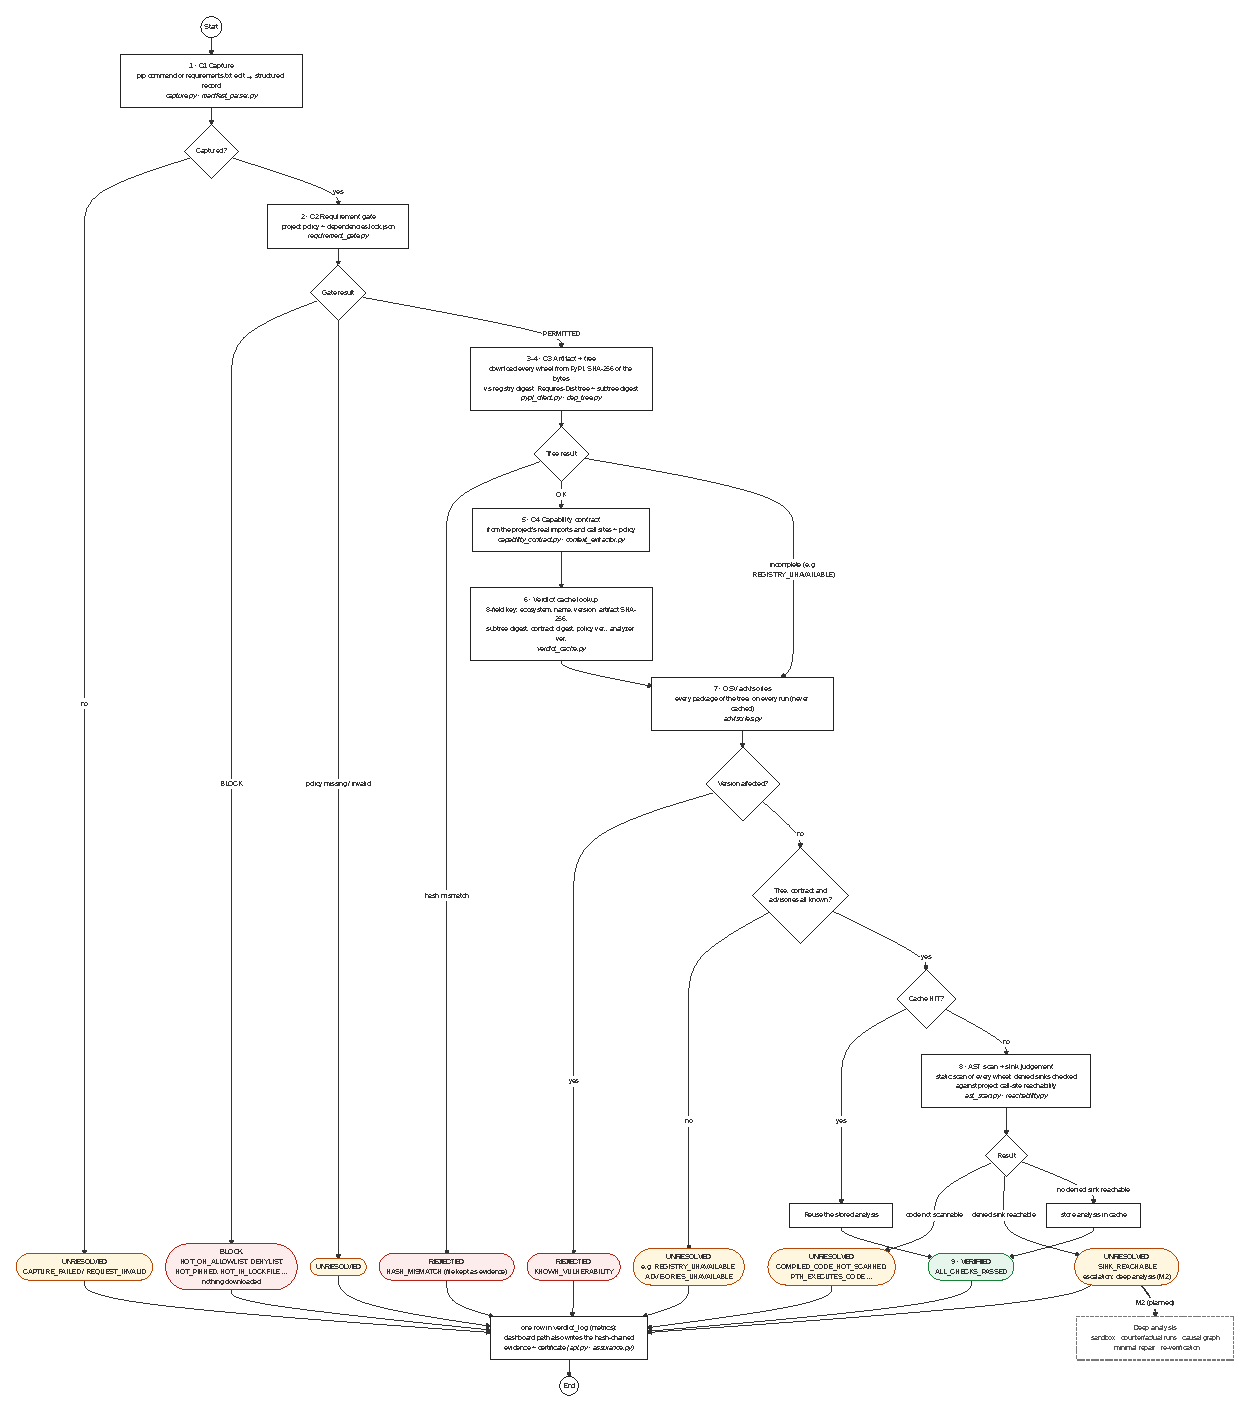
\includegraphics[height=0.88\textheight]{figures/diagrams/cavr-activity.pdf}
\caption{Activity diagram of the CAVR fast gate, \texttt{verify\_request} in \texttt{backend/cavr/pipeline.py}. Numbers follow the stage order in the code; the dashed element is planned (M2).}
\label{fig:cavr-activity}
\end{figure}

Figure~\ref{fig:cavr-activity} follows \texttt{verify\_request} stage by stage. The request is captured as a structured record (1) and checked by the requirement gate against the project policy and the lockfile (2); a request that is not permitted ends as \texttt{BLOCK} before anything is downloaded. Every wheel of the dependency tree is then downloaded from PyPI and its SHA-256 compared with the registry digest, and the tree and its subtree digest are built from the real \texttt{Requires-Dist} metadata (3--4); a mismatch is \texttt{REJECTED}. The capability contract is inferred from the project's own imports and call sites (5); only then can the 8-field cache key be formed and looked up (6), because it contains the contract digest. OSV is asked for every package of the tree on every run, also on a cache hit (7): an affected version is \texttt{REJECTED}, and any unknown input (registry, contract or advisories) is \texttt{UNRESOLVED}. On a cache miss the wheels are scanned statically and every denied sink is judged against the project's call-site reachability (8). A reachable denied sink is not treated as proven malicious: the verdict is \texttt{UNRESOLVED} with an escalation to M2 deep analysis. Only a complete analysis is stored in the cache. Every verdict writes one row to the verdict log; requests made from the dashboard also write the hash-chained evidence and the certificate.

% ======================================================================
% (3) Ch 5 "Process / Behavior Design": CAVR sequence
% ======================================================================
\begin{figure}[htbp]
\centering
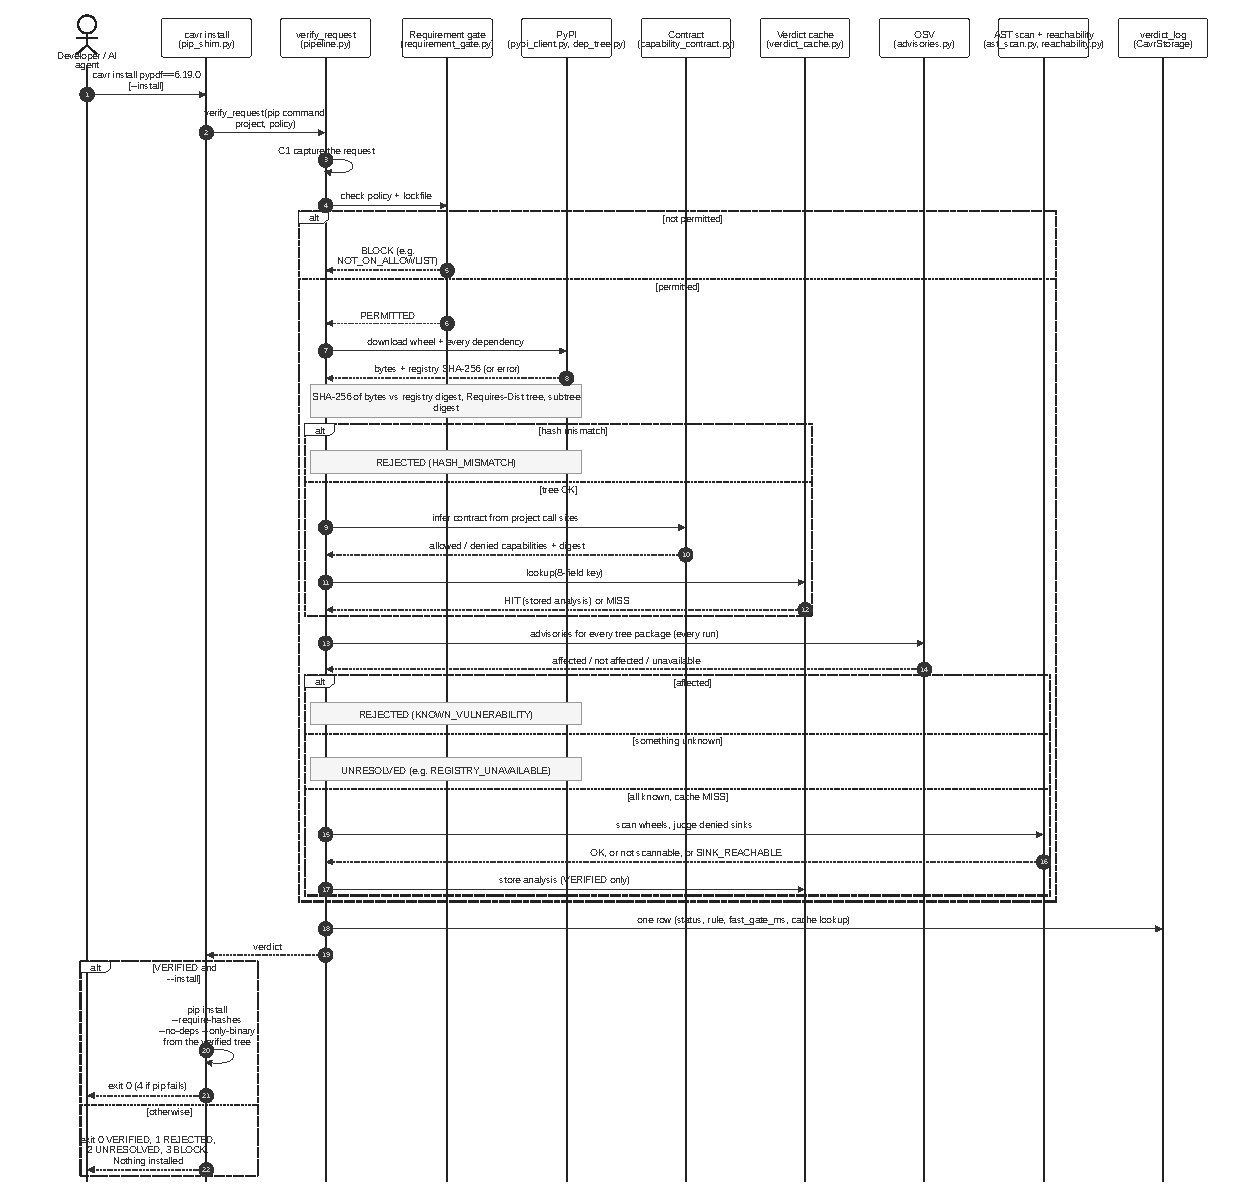
\includegraphics[width=\textwidth]{figures/diagrams/cavr-sequence.pdf}
\caption{Sequence of a \texttt{cavr install} request (\texttt{pip\_shim.py}) through \texttt{verify\_request} and its collaborators, with the wrapper's exit codes.}
\label{fig:cavr-sequence}
\end{figure}

Figure~\ref{fig:cavr-sequence} shows the same pipeline as messages between components. The wrapper never passes the user's arguments to pip; it only calls \texttt{verify\_request} and prints the verdict (exit code 0 \texttt{VERIFIED}, 1 \texttt{REJECTED}, 2 \texttt{UNRESOLVED}, 3 \texttt{BLOCK}). Only with \texttt{--install} and a \texttt{VERIFIED} verdict does it write a requirements file of the verified tree with \texttt{--hash=sha256} pins and run pip with \texttt{--require-hashes --no-deps --only-binary :all:}, so pip cannot install a different file, an unverified dependency or an sdist; a pip failure gives exit code 4.

% ======================================================================
% (4) Ch 5 "Process / Behavior Design": CAVR state
% ======================================================================
\begin{figure}[htbp]
\centering
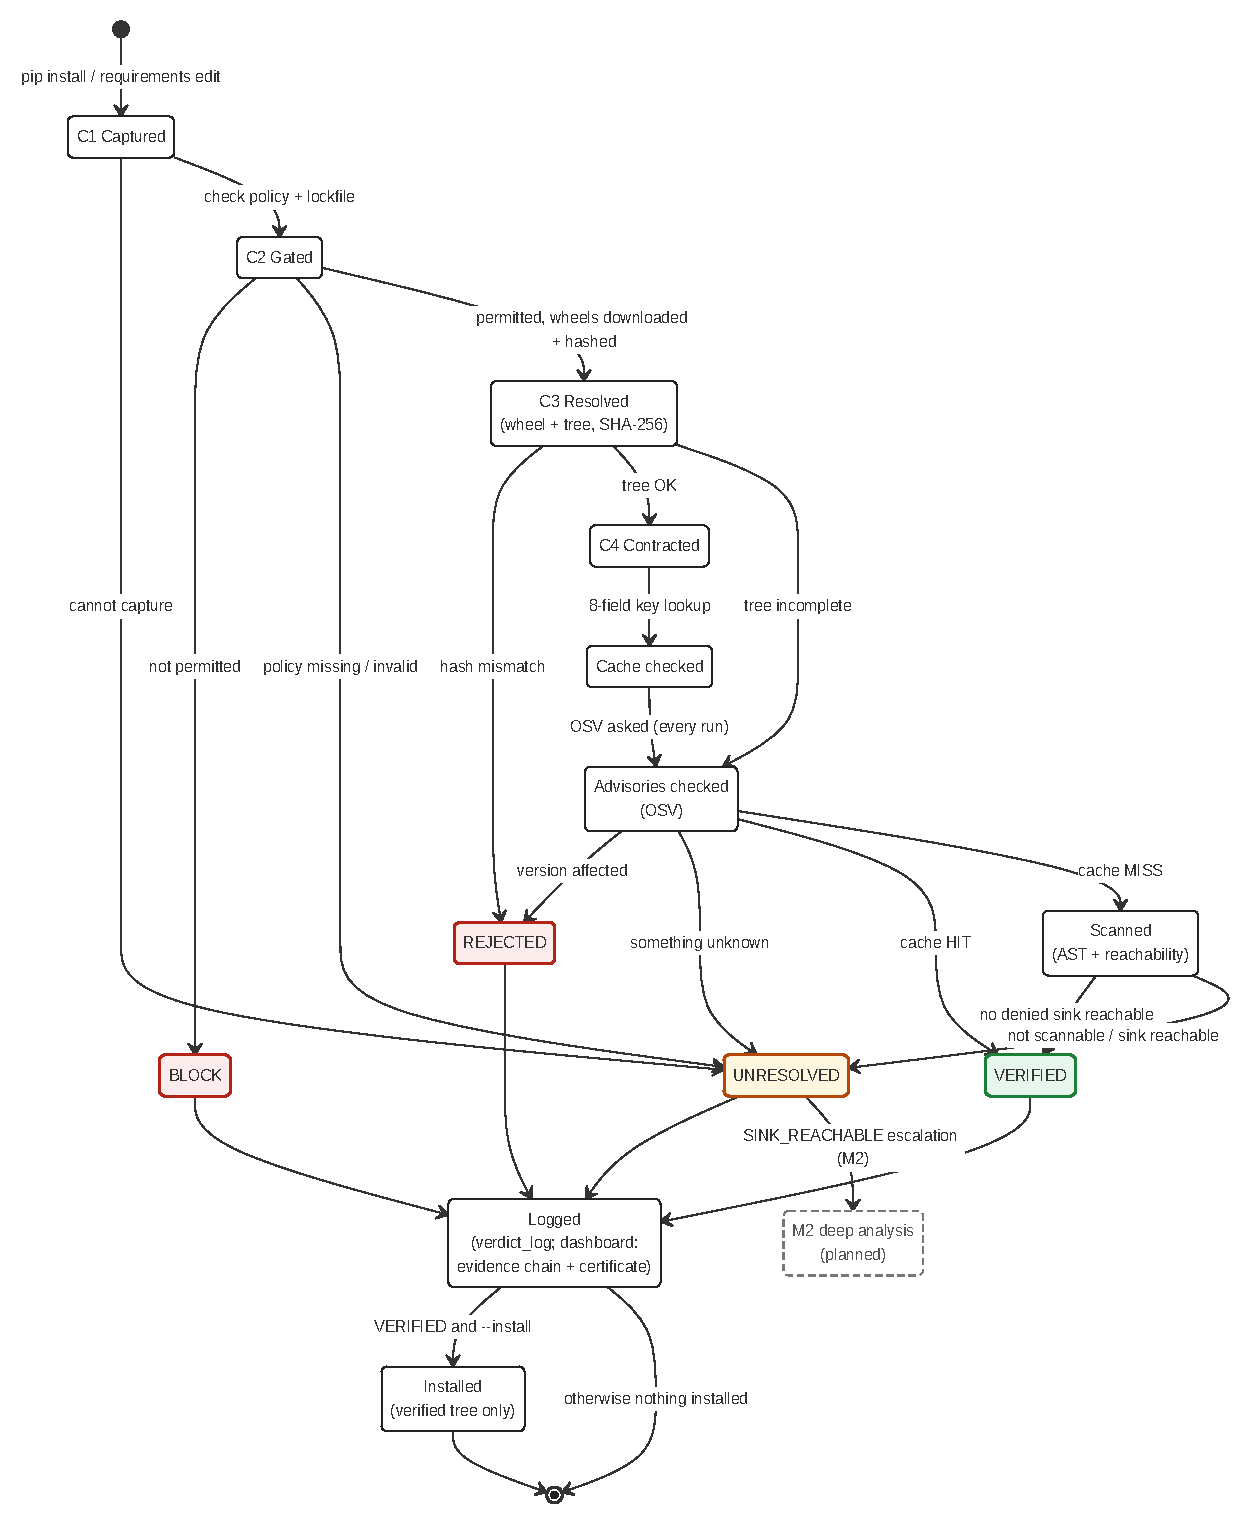
\includegraphics[width=0.85\textwidth]{figures/diagrams/cavr-state.pdf}
\caption{Lifecycle of a CAVR request. All four verdicts are logged; only a \texttt{VERIFIED} request with \texttt{--install} is installed.}
\label{fig:cavr-state}
\end{figure}

Figure~\ref{fig:cavr-state} shows the states of one request. \texttt{REJECTED} is reached only with positive evidence of a problem (a hash mismatch or an OSV advisory); every gap in the evidence leads to \texttt{UNRESOLVED}, which is never treated as a pass. \texttt{UNRESOLVED} with \texttt{SINK\_REACHABLE} is the state that M2 deep analysis will take over.

% ======================================================================
% (5) Ch 5 "Data Design": ERD
% ======================================================================
\begin{figure}[htbp]
\centering
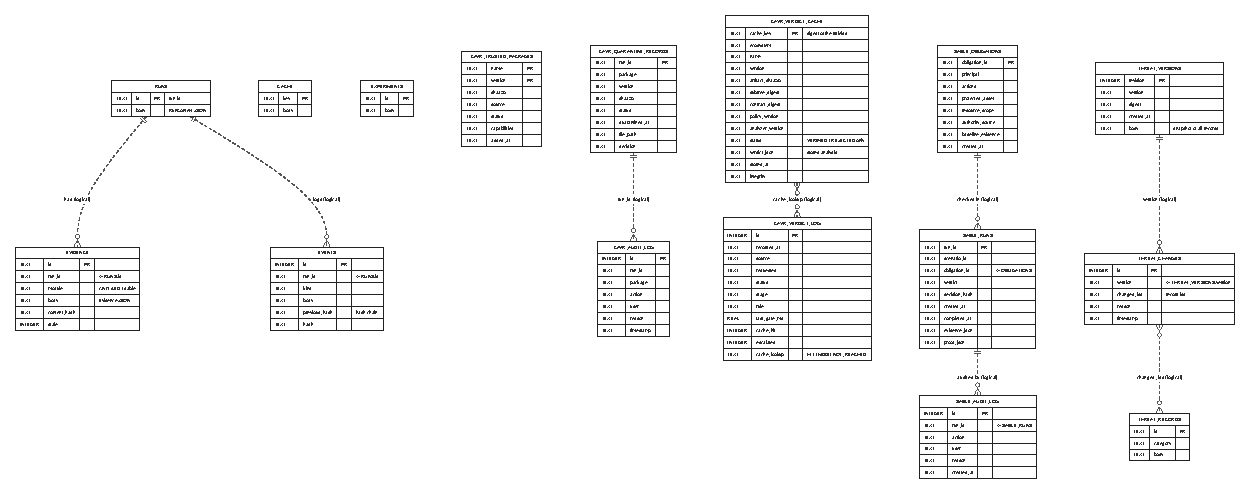
\includegraphics[width=\textwidth]{figures/diagrams/erd.pdf}
\caption{Entity--relationship diagram of the SQLite stores (\texttt{db/storage.py}, \texttt{cavr/storage.py}, \texttt{sable/storage.py}, \texttt{threat\_repo/repository.py}). Dashed relationships are logical: the code writes the same identifier into both tables but declares no foreign keys.}
\label{fig:asent-erd}
\end{figure}

Figure~\ref{fig:asent-erd} shows the persistent data. The shared run store keeps each run as a \texttt{RunContext} JSON document, the module evidence bound to it (with a content hash and a stale flag) and the run events as a hash chain. The CAVR store holds the M1 \texttt{verdict\_cache}, keyed by a digest of the eight key fields and storing only complete analyses with an integrity value, and the \texttt{verdict\_log}, one row per request, from which the cache hit rate and the p50/p95 latency are computed; the trusted-package, quarantine and audit tables come from the earlier prototype. The SABLE store holds registered obligations, SABLE runs and their audit log, and the threat repository versions its records so that every change has a version and a reason. Integrity is enforced by the code (shared identifiers, content hashes, hash chains) rather than by declared foreign keys.

% ======================================================================
% (6) Ch 8 CI/CD section (chapter9_development_evidence.tex)
% ======================================================================
\begin{figure}[htbp]
\centering
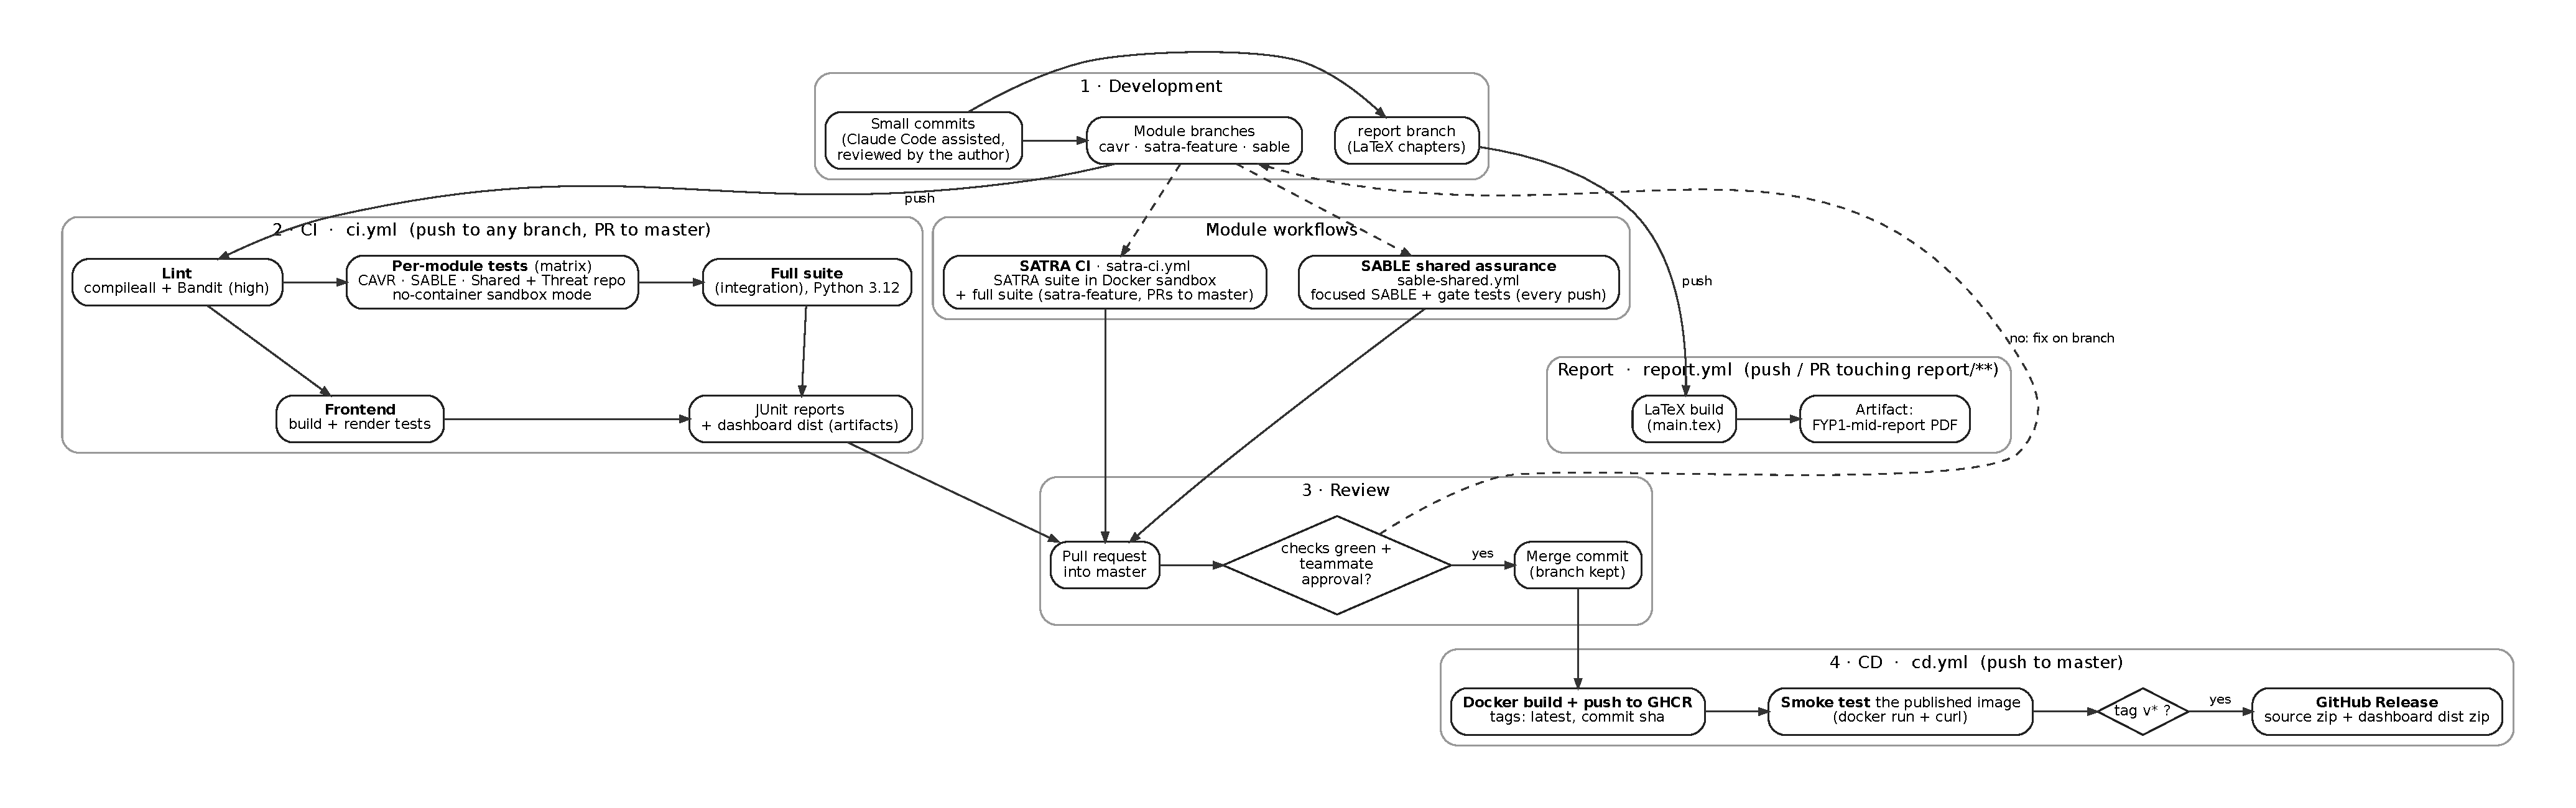
\includegraphics[width=\textwidth]{figures/diagrams/cicd.pdf}
\caption{Development and CI/CD workflow of the repository (\texttt{.github/workflows}: \texttt{ci.yml}, \texttt{satra-ci.yml}, \texttt{sable-shared.yml}, \texttt{cd.yml}, \texttt{report.yml}).}
\label{fig:asent-cicd}
\end{figure}

Figure~\ref{fig:asent-cicd} shows how code reaches \texttt{master}. Each member works on a module branch with small commits. Every push runs CI (\texttt{ci.yml}): lint (\texttt{compileall} and Bandit at high severity), per-module test jobs for CAVR, SABLE and the shared/threat-repository code, the full integration suite on Python~3.12, and the frontend build with render tests, keeping JUnit reports as artifacts. SATRA-RV has its own workflow that runs its suite in the Docker sandbox, and SABLE has a focused shared-assurance workflow. A pull request is merged with a merge commit only when the checks are green and a teammate has approved it. A push to \texttt{master} runs CD (\texttt{cd.yml}): the Docker image is built and pushed to GitHub Container Registry and the published image is smoke-tested; a \texttt{v*} tag also creates a GitHub Release. Changes under \texttt{report/} build this report as a PDF artifact.
